%=========================================================================
% fig-intro-vision
%=========================================================================

%\begin{figure}

  \centering
  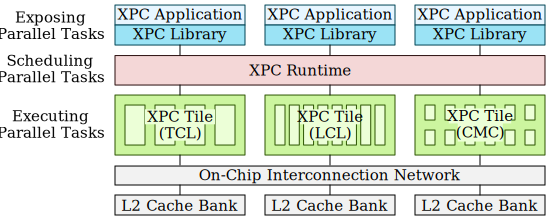
\includegraphics[width=\tw]{intro-vision.svg.pdf}

  \caption{\textbf{XPC Architecture Overview --} XPC applications use an
    XPC parallel programming library to expose fine-grain parallel tasks.
    A software runtime is used to facilitate adaptive task distribution
    across XPC tiles based on statistics collected during profiling. The
    heterogeneous XPC tiles are specialized for various forms of
    parallelism, but all XPC tiles have a common ISA.}

  \label{fig-intro-vision}

%\end{figure}
